\chapter{慢病风险因素}

慢性病的风险评估主要通过参检夫妇自报是否患有或曾经患有各种慢性疾病,测量血压、血糖、肝功能(谷丙转氨酶,ALT)、肾功能(肌酐,Cr)及甲状腺功能(促甲状腺激素,TSH)等临床实验室指标来识别是否患有可能增加出生缺陷等不良妊娠结局发生风险的慢性疾病。

\section{慢性病自报患病情况}

孕前健康检查询问了参检夫妇是否患有或曾经患过下列七种主要慢性非传染性疾病:高血压、心脏病、糖尿病、癫痫、甲状腺疾病、慢性肾炎、肿瘤。

在女方参检对象中,自报患有或曾经患有至少一种上述慢性病的比例(简称自报患病率)为None\%。男方参检对象中,自报慢性病患病率为1.96\%。2015年深圳市各地区女方及男方自报慢性病患病情况如下图、表所示。其中,女方自报慢病患病率顺位前三名的地区分别为【None】,其自报慢病患病率分别为5.81\%、4.57\%及4.41\%;【待实现】男方自报慢病患病率顺位前三名的地区分别为【[('440304',), ('440306',), ('440307',)]】,其自报慢病患病率分别为4.83\%、3.84\%及3.76\%。【待实现】


\begin{figure}[htbp]
	\centering
	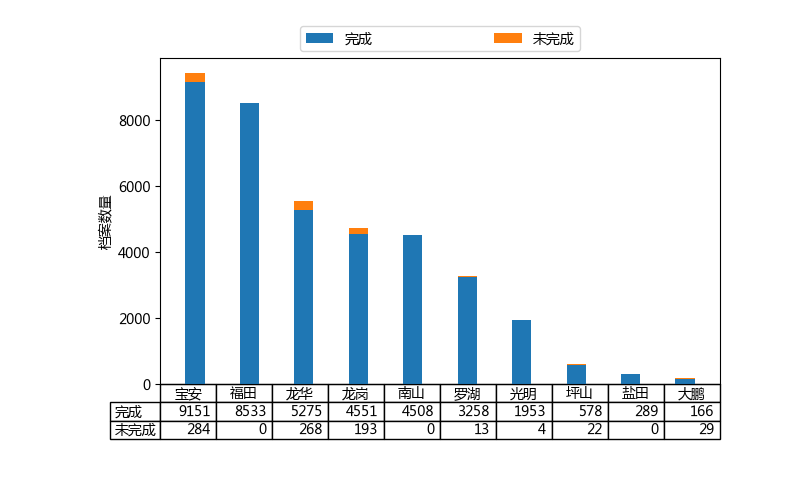
\includegraphics[width=1\textwidth]{1.png}
	\caption{'占位图'}
	\label{}
\end{figure}


对男女双方自报慢性病的种类进行统计分析发现,在女性参检人群中,排在前五位的分别为【(hypertension\_A, heart\_disease\_A, diabetes\_A, epilepsy\_A, thyroid\_disease\_A, chronic\_nephritis\_A, swelling\_A);None】,其患病率分别为None\%、None\%, None\%, None\%, None\%, None\%;男性参检人群中,排在前五位的分别为【(hypertension, heart\_disease, diabetes, epilepsy, thyroid\_disease, chronic\_nephritis, swelling); [('1', None, None, None, None, None, None), (None, None, None, None, '1', None, None), (None, None, '1', None, None, None, None), (None, None, None, None, None, '1', None), (None, '1', None, None, None, None, None)]】,其患病率分别为0.80\%、0.47\%, 0.19\%, 0.16\%, 0.11\%, 0.80\%。2015年深圳市女方及男方自报主要慢性病种类的情况如下图、表所示。

 

与2014年参检服务对象自报的慢性病种类情况相比,2015年全市女方、男方自报顺位前三位的慢性病种类与2014年基本相同。2015年与2014年深圳市自报的主要慢性病种类对比情况如下图所示。

 

\section{慢性病相关测量指标检测情况}

为识别是否患有可能影响出生缺陷等不良妊娠结局的慢性疾病,孕前健康检查对女方进行了血压的测量和血糖、甲状腺功能(促甲状腺激素,TSH)、肝功能(谷丙转氨酶,ALT)、肾功能(肌酐,Cr)等实验室指标的检测,对男方进行了血压测量、肝功能(谷丙转氨酶,ALT)和肾功能(肌酐,Cr)等实验室指标的检测。

\subsection{血压测量与高血压}

根据血压测量结果,女方参检对象的高血压患病率为None\%,男方参检对象的高血压患病率为9.86\%,男性高血压患病率普遍高于女性患病率。按照血压测量结果界定的高血压患病率显著高于高血压自报患病率。不同地区男女双方高血压患病率情况如下图所示,女方高血压患病率顺位前三位的分别为【None】,检出率分别为None\%, None\%,None\%,;男方高血压患病率顺位前三位的分别为【[('440306',), ('440304',), ('440305',)]】,高血压检出率分别为3.85\%, 2.15\%,1.09\%。

2015年与2014年高血压患病率比较如下图。

 

\subsection{血糖检测与糖尿病初筛异常}

根据血糖检测结果,将空腹血糖(FPG)≥ 6.10mmol/L界定为糖尿病初筛异常 。按此界定,女方参检对象的糖尿病初筛异常率为5.26\%,高/低于2014年【2014年的数据为:4.35\%】。糖尿病初筛异常者需要做进一步的检查以确诊,并根据诊断结果提供专业咨询指导。不同地区女性空腹血糖筛查异常情况如下图所示。女方空腹血糖筛查异常率顺位前三位的分别为【[('440304',), ('440306',), ('440305',)]】,检出率分别为15.91\%、3.18\%和3.15\%。【待支持按区计算】与2014年相比,福田区、宝安区、光明区、龙岗区、平山新区、龙华区及南山区空腹血糖筛查异常率均有所上升,而盐田区有明显降低。

将FPG≥7.00mmol/L或自报有糖尿病病史定义为糖尿病,则女方参检对象糖尿病检出率为None\%,高于2014年的None\%。不同地区女性糖尿病检出率如下图所示。女方糖尿病检出率顺位前三位的分别为【None】,检出率分别为4.77\%、1.01\%和0.74\%。【待支持】与2014年相比,福田区、坪山新区、光明新区、罗湖区糖尿病检出率均有所上升,而宝安区、南山区及龙华新区则有所降低。

 

\subsection{促甲状腺激素检测异常}

根据促甲状腺激素(TSH)检测结果,TSH<0.44μmol/L 或TSH>3.45界定为TSH异常 。按此界定,女方参检对象的甲状腺功能异常率为None\%),明显高于其自报甲状腺疾病的患病率。甲状腺功能异常者需要做进一步的检查以确诊,并根据诊断结果提供专业咨询指导。从各区的分布情况来看,女方甲状腺异常率顺位前三位的分别为【[('440306',), ('440304',), ('440305',)]】,检出率分别为22.43\%、19.45\%和18.77\%。【未实现】不同地区女性甲状腺疾病检测异常情况如下图所示。

 

与2014年相比,女性甲状腺功能筛查异常的各区平均值变化不大。宝安区、南山区、光明新区、盐田区2015年度女性甲状腺功能筛查异常率显著高于2014年度的异常率。

 

\subsection{谷丙转氨酶检测与肝功能异常}

谷丙转氨酶(ALT)升高提示肝细胞损伤,根据ALT检测结果,ALT>45U/L界定为肝功能异常 。按照此标准,结果显示女方参检对象肝功能异常率为None\%,男方参检对象肝功能异常率为0.17\%。男方参检对象肝功能异常率明显高于女方。女方肝功能异常率顺位前三位的分别为【None】,检出率分别为3.46\%、3.44\%和3.12\%;【未实现】男方肝功能异常率顺位前三位的分别为【[('440304',), ('440306',), ('440305',)]】,检出率分别为23.23\%、20.47\%和19.71\%。

 

与2014年相比,2015年女性肝功能筛查异常率坪山新区、龙岗区、宝安区有明显减少,南山区、大鹏新区、罗湖区、福田区男女方肝功能异常率比去年有所升高。详见2014与2015年男女性肝功能筛查异常率比较图。

 

\subsection{肌酐检测与肾功能异常}

根据Cr检测结果,女方Cr >73μmol/L或者Cr <41μmol/L界定为肾功能异常,男方Cr >97μmol/L或者Cr <57μmol/L界定为肾功能异常 。按此界定,女方参检对象肾功能异常率为None\%,男方参检对象肾功能异常率为0.31\%,女方参检对象肾功能异常率明显低于男方。女方肾功能异常率顺位前三位的分别为【None】,检出率分别为28.18\%、10.74\%和8.97\%;【未实现】男方肾功能异常率顺位前三位的分别为【[('440304',), ('440306',), ('440307',)]】,检出率分别为53.67\%、18.41\%和16.01\%。【未实现】与2014年相比,宝安区、罗湖区、南山区和龙华区女性和男性的肾功能异常率明显降低,但福田区的女性和男性肾功能异常率却比去年有明显上升。2015年和2014年肾功能异常率比较结果如下图所示。

